\documentclass{article}

\usepackage[fontsize=13pt]{scrextend}
\usepackage{geometry}
\usepackage{multicol}
\usepackage{lmodern} % For scalable Computer Modern fonts % Ensures proper font encoding
\usepackage{color}
\usepackage{helvet}  % For changing fonts

\usepackage{soul}  % For highlighting

\geometry{
  a4paper,
  left=25mm,
  right=25mm,
  top=25mm,
  bottom=25mm,
  heightrounded,
}



\usepackage{lastpage} % Required to determine the last page number for the footer

\usepackage{graphicx} % Required to insert images

\setlength\parindent{0pt} % Removes all indentation from paragraphs

\usepackage[most]{tcolorbox} % Required for boxes that split across pages

\usepackage{booktabs} % Required for better horizontal rules in tables

\usepackage{listings} % Required for insertion of code

\usepackage{etoolbox} % Required for if statements

%----------------------------------------------------------------------------------------
%	MARGINS
%----------------------------------------------------------------------------------------

\usepackage{geometry} % Required for adjusting page dimensions and margins

\geometry{
	paper=a4paper, % Change to letterpaper for US letter
	top=3cm, % Top margin
	bottom=3cm, % Bottom margin
	left=2.5cm, % Left margin
	right=2.5cm, % Right margin
	headheight=14pt, % Header height
	footskip=1.4cm, % Space from the bottom margin to the baseline of the footer
	headsep=1.2cm, % Space from the top margin to the baseline of the header
	%showframe, % Uncomment to show how the type block is set on the page
}

%----------------------------------------------------------------------------------------
%	FONT
%----------------------------------------------------------------------------------------

\usepackage[utf8]{inputenc} % Required for inputting international characters
\usepackage[T1]{fontenc} % Output font encoding for international characters

\usepackage[sfdefault,light]{roboto} % Use the Roboto font

%----------------------------------------------------------------------------------------
%	HEADERS AND FOOTERS
%----------------------------------------------------------------------------------------

\usepackage{fancyhdr} % Required for customising headers and footers

\pagestyle{fancy} % Enable custom headers and footers

\lhead{\small\assignmentClass\ifdef{\assignmentClassInstructor}{\ (\assignmentClassInstructor):}{}\ \assignmentTitle} % Left header; output the instructor in brackets if one was set
\chead{} % Centre header
\rhead{\small\ifdef{\assignmentAuthorName}{\assignmentAuthorName}{\ifdef{\assignmentDueDate}{Due\ \assignmentDueDate}{}}} % Right header; output the author name if one was set, otherwise the due date if that was set

\lfoot{} % Left footer
\cfoot{\small Page\ \thepage\ of\ \pageref{LastPage}} % Centre footer
\rfoot{} % Right footer

\renewcommand\headrulewidth{0.5pt} % Thickness of the header rule

%----------------------------------------------------------------------------------------
%	MODIFY SECTION STYLES
%----------------------------------------------------------------------------------------

\usepackage{titlesec} % Required for modifying sections
\usepackage{longtable}
%------------------------------------------------
% Section

\titleformat
{\section} % Section type being modified
[block] % Shape type, can be: hang, block, display, runin, leftmargin, rightmargin, drop, wrap, frame
{\Large\bfseries} % Format of the whole section
{\assignmentQuestionName~\thesection} % Format of the section label
{6pt} % Space between the title and label
{} % Code before the label

\titlespacing{\section}{0pt}{0.5\baselineskip}{0.5\baselineskip} % Spacing around section titles, the order is: left, before and after

%------------------------------------------------
% Subsection

\titleformat
{\subsection} % Section type being modified
[block] % Shape type, can be: hang, block, display, runin, leftmargin, rightmargin, drop, wrap, frame
{\itshape} % Format of the whole section
{(\alph{subsection})} % Format of the section label
{4pt} % Space between the title and label
{} % Code before the label

\titlespacing{\subsection}{0pt}{0.5\baselineskip}{0.5\baselineskip} % Spacing around section titles, the order is: left, before and after

\renewcommand\thesubsection{(\alph{subsection})}

%----------------------------------------------------------------------------------------
%	CUSTOM QUESTION COMMANDS/ENVIRONMENTS
%----------------------------------------------------------------------------------------

% Environment to be used for each question in the assignment
\newenvironment{question}{
	\vspace{0.5\baselineskip} % Whitespace before the question
	\section{} % Blank section title (e.g. just Question 2)
	\lfoot{\small\itshape\assignmentQuestionName~\thesection~continued on next page\ldots} % Set the left footer to state the question continues on the next page, this is reset to nothing if it doesn't (below)
}{
	\lfoot{} % Reset the left footer to nothing if the current question does not continue on the next page
}

%------------------------------------------------

% Environment for subquestions, takes 1 argument - the name of the section
\newenvironment{subquestion}[1]{
	\subsection{#1}
}{
}

%------------------------------------------------

% Command to print a question sentence
\newcommand{\questiontext}[1]{
	\textbf{#1}
	\vspace{0.5\baselineskip} % Whitespace afterwards
}

%------------------------------------------------

% Command to print a box that breaks across pages with the question answer
\newcommand{\answer}[1]{
	\begin{tcolorbox}[breakable, enhanced]
		#1
	\end{tcolorbox}
}

%------------------------------------------------

% Command to print a box that breaks across pages with the space for a student to answer
\newcommand{\answerbox}[1]{
	\begin{tcolorbox}[breakable, enhanced]
		\vphantom{L}\vspace{\numexpr #1-1\relax\baselineskip} % \vphantom{L} to provide a typesetting strut with a height for the line, \numexpr to subtract user input by 1 to make it 0-based as this command is
	\end{tcolorbox}
}

%------------------------------------------------

% Command to print an assignment section title to split an assignment into major parts
\newcommand{\assignmentSection}[1]{
	{
		\centering % Centre the section title
		\vspace{2\baselineskip} % Whitespace before the entire section title
		
		\rule{0.8\textwidth}{0.5pt} % Horizontal rule
		
		\vspace{0.75\baselineskip} % Whitespace before the section title
		{\LARGE \MakeUppercase{#1}} % Section title, forced to be uppercase
		
		\rule{0.8\textwidth}{0.5pt} % Horizontal rule
		
		\vspace{\baselineskip} % Whitespace after the entire section title
	}
}

%----------------------------------------------------------------------------------------
%	TITLE PAGE
%----------------------------------------------------------------------------------------

\author{\textbf{\assignmentAuthorName}} % Set the default title page author field
\date{} % Don't use the default title page date field

\title{
	\thispagestyle{empty} % Suppress headers and footers
	\vspace{0.2\textheight} % Whitespace before the title
	\textbf{\assignmentClass:\ \assignmentTitle}\\[-4pt]
	\ifdef{\assignmentDueDate}{{\small Due\ on\ \assignmentDueDate}\\}{} % If a due date is supplied, output it
	\ifdef{\assignmentClassInstructor}{{\large \textit{\assignmentClassInstructor}}}{} % If an instructor is supplied, output it
	\vspace{0.32\textheight} % Whitespace before the author name
}

\usepackage[utf8]{inputenc}
\usepackage[T1]{fontenc}
\usepackage{lmodern}
\usepackage{booktabs}
\usepackage{xcolor}
\usepackage{tikz}
\usepackage{pgfplots}
\usepackage{graphicx}

\usepackage{amsmath}


\usepackage{amsfonts}
\usepackage{amssymb}

\usepackage{tabularx}



\usepackage{hyperref}
\usepackage{listings}
\usepackage{booktabs}
\usepackage{tabularray}
\usepackage{multirow}
\usepackage{float}
\usepackage{lastpage}
\usepackage{tcolorbox}
\usepackage{titlesec}

\usepackage{etoolbox}


\usepackage[T1]{fontenc}

\usepackage{enumitem}
\usepackage{hyperref}
\usepackage{babel}
\usepackage{graphicx}
\usepackage{url}
\usepackage{amsmath}
\usepackage{pgfplots}
\pgfplotsset{compat=1.17}
\usepackage{amsmath}
\usepackage{hyperref}
\usepackage{fontawesome}
\usepackage{float}    % For enforcing image position with [H]


\makeatletter
\patchcmd{\@zfancyhead}{\fancy@reset}{\f@nch@reset}{}{}
\patchcmd{\@set@em@up}{\f@ncyolh}{\f@nch@olh}{}{}
\patchcmd{\@set@em@up}{\f@ncyolh}{\f@nch@olh}{}{}
\patchcmd{\@set@em@up}{\f@ncyorh}{\f@nch@orh}{}{}
\makeatother

\pgfplotsset{compat=newest}

% Colors from structure.tex
\definecolor{secondaryColor}{RGB}{0,0,0}
\definecolor{accentColor1}{RGB}{255,87,34}
\definecolor{accentColor3}{RGB}{63,81,181}
\definecolor{textColor}{RGB}{33,33,33}
\definecolor{primaryColor}{RGB}{34, 45, 101}
\definecolor{accentColor2}{RGB}{46, 117, 182}
\definecolor{backgroundColor}{RGB}{245, 245, 245}
\definecolor{fitcolor}{RGB}{0,128,0}
\definecolor{okaycolor}{RGB}{255,165,0}
\definecolor{notfitcolor}{RGB}{255,0,0}



\definecolor{sectioncolor}{RGB}{0,0,100}  % Deep blue for main headings
\definecolor{subcolor}{RGB}{100,0,100}  % Purple for subheadings
\definecolor{lightRed}{RGB}{255,200,200}  % Light red for section underline
\definecolor{lightPink}{RGB}{255,220,220}  % Light pink for subsection underline


\newcommand{\highlight}[1]{\textsf{\textbf{#1}}}  % For highlighting key terms in sans-serif bold
% Custom underline command
\newcommand{\customunderline}[2]{%
  \par\noindent\rule{0pt}{2ex}\vspace{-0.5in} % Adjust the space here
  \colorbox{#1}{\makebox[\linewidth]{#2}}\par
}

% Section format
\titleformat{\section}
  {\color{sectioncolor}\Huge\bfseries\sffamily}  % Sans-serif, huge, bold, blue
  {}
  {0pt}
  {}
  
 

% Subsection format
\titleformat{\subsection}
  {\color{subcolor}\Large\bfseries\sffamily}  % Sans-serif, large, bold, purple
  {}
  {0pt}
  {}

% % Adjust spacing
% \titlespacing*{\section}{0pt}{3.5ex plus 1ex minus .2ex}{2.3ex plus .2ex}
% \titlespacing*{\subsection}{0pt}{3.25ex plus 1ex minus .2ex}{1.5ex plus .2ex}


% % Modify the question environment to include color
% \renewenvironment{question}{
%   \vspace{0.5\baselineskip}
%   \section{}
%   \lfoot{\small\itshape\color{primaryColor}\assignmentQuestionName~\thesection~continued on next page\ldots}
% }{
%   \lfoot{}
% }

% Modify the answer command to include color
\renewcommand{\answer}[1]{
  \begin{tcolorbox}[
    breakable,
    enhanced,
    colback=backgroundColor,
    colframe=primaryColor,
    coltitle=white,
    title=Answer
  ]
    #1
  \end{tcolorbox}
}

% Modify the assignmentSection command to include color
\renewcommand{\assignmentSection}[1]{
  {
    \centering
    \vspace{2\baselineskip}
    
    \color{primaryColor}\rule{0.8\textwidth}{0.5pt}
    
    \vspace{0.75\baselineskip}
    {\LARGE\color{primaryColor}\MakeUppercase{#1}}
    
    \color{primaryColor}\rule{0.8\textwidth}{0.5pt}
    
    \vspace{\baselineskip}
  }
}

\definecolor{deepblue}{RGB}{0,76,153}
\definecolor{lightblue}{RGB}{173,216,230}
\definecolor{orange}{RGB}{255,165,0}

% Custom title format
\titleformat{\section}
  {\color{deepblue}\normalfont\Large\bfseries}
  {\color{deepblue}\thesection}{1em}{}

% Custom enumeration
\setlist[enumerate,1]{label=\color{orange}\arabic*.,font=\bfseries}


% Modify headers and footers to include color
\lhead{\small\color{primaryColor}\assignmentClass\ifdef{\assignmentClassInstructor}{\ (\assignmentClassInstructor):}{Ayush Kumar Mishra}\ \assignmentTitle}
\rhead{\small\color{secondaryColor}\ifdef{\assignmentAuthorName}{\assignmentAuthorName}{\ifdef{\assignmentDueDate}{Due\ \assignmentDueDate}{}}}
\cfoot{\small\color{primaryColor}Page\ \thepage\ of\ \pageref{LastPage}}

\renewcommand\headrulewidth{0.5pt}
\renewcommand{\headrule}{\hbox to\headwidth{\color{primaryColor}\leaders\hrule height \headrulewidth\hfill}}

\hypersetup{
    colorlinks=true,
    linkcolor=primaryColor,
    filecolor=accentColor1,      
    urlcolor=accentColor3,
    pdftitle={Machine Learning phase-2 Submission},
    pdfpagemode=FullScreen,
}

\title{\textcolor{primaryColor}{\Huge\textbf{Machine Learning phase-2 Submission}}}
\author{\textcolor{secondaryColor}{\Large Ayush Kumar Mishra}}
\date{\textcolor{secondaryColor}{\today}}

\begin{document}

\maketitle

\newpage
\section*{Dashboard}
  \begin{center}
        \color{red}\rule{1\linewidth}{1mm}
    \end{center}
\begin{center}
\vspace{2in}
    {\Huge  For seeing all the code live interactively, \\
    \vspace{1.5in}
    Website  \href{https://krishi-ai.onrender.com/}{Website}}\\
    
    \vspace{0.7in}
   \textbf{ \href{https://krishi-ai.onrender.com/}{https://krishi-ai.onrender.com/}}
   \vspace{l.5in}
   Github Reposotory \href{https://github.com/Ayush-mishra-0-0/cs550/}\\

\end{center}

\newpage
\tableofcontents


\newpage

\begin{document}
\maketitle

% \begin{center}
%     \section*{\textcolor{teal}{\huge{Krishi.ai \href{https://krishi-ai.onrender.com/}{\faExternalLink}}}}
%     \section*{\textcolor{teal}{\large{Repo \href{https://github.com/shivamlth27/Krishi_ai}{\faExternalLink}}}}
% \end{center}



\section{1. Project Directory}
{
    To begin with the project, we first created a directory structure to organize our work. The directory structure is as follows:
    \begin{itemize}
        \item \textbf{Data:} This directory contains the datasets used for training and validation. It includes subdirectories for each dataset, along with the necessary annotations and labels.{
            \begin{center}
                \fbox{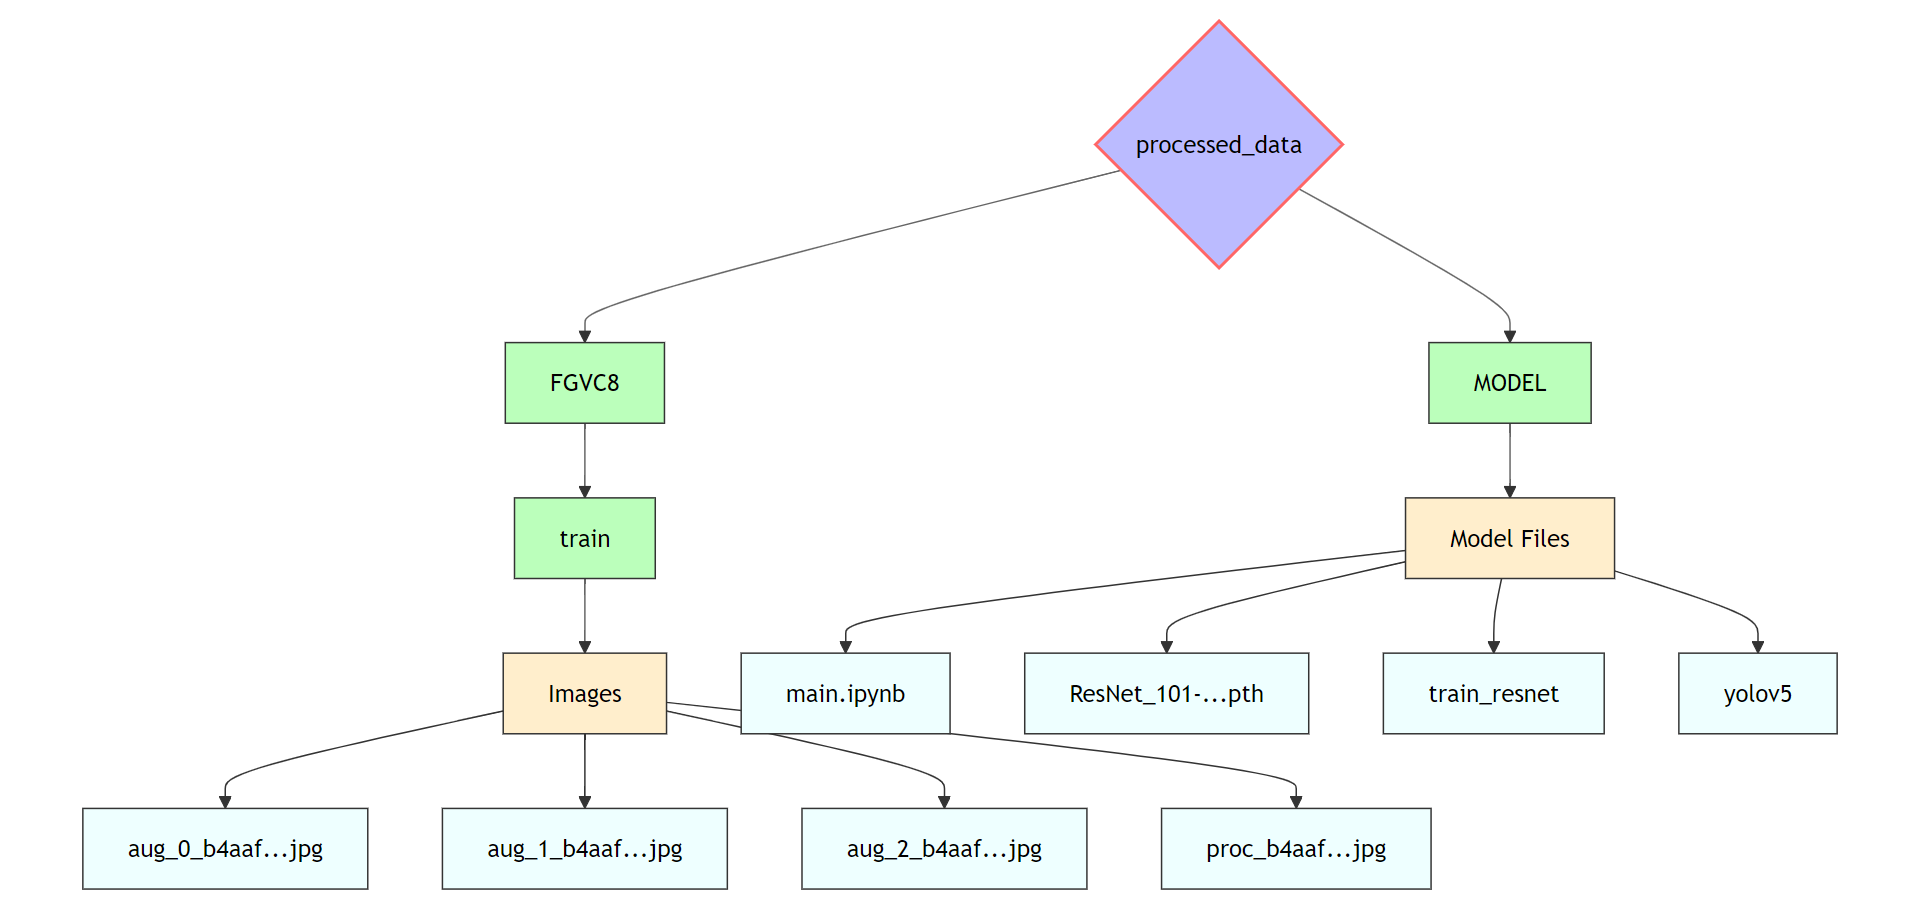
\includegraphics[width=0.7\textwidth]{images/image6(flowchart1).png}}
                \\
                \vspace{0.1in}
                \caption{This is flowchart for model and data directory.}
            \end{center}
            \begin{center}
                \fbox{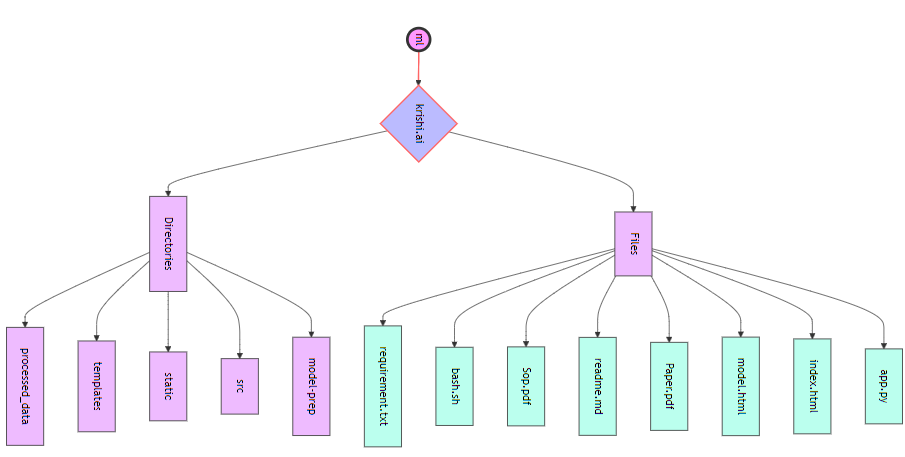
\includegraphics[width=0.7\textwidth]{images/image7(flowchart2).png}}
                
                \\
                \vspace{0.1in}
                \caption{This is flowchart for flask server and website directory.}
            \end{center}

        }
    \end{itemize}
}
\setlist[enumerate,1]{label=\color{orange}\arabic*.,font=\bfseries}


\section{Project Workflow}

The project workflow was divided into several phases, each focusing on a specific aspect of the project. The workflow included the following steps:

\begin{enumerate}[leftmargin=*]
 
\item \textbf{Data Collection:} 
\begin{tcolorbox}[colback=lightblue!10,colframe=deepblue,title=Datasets]
As stated in the paper, we used three different datasets for training and validation. These datasets contained images of plant leaves affected by various diseases.
\end{tcolorbox}

\item \textbf{Data Preprocessing and Augmentation:} 
In this step, we performed the following operations:

\begin{enumerate}[label=\alph*,leftmargin=*]
    \item \textcolor{deepblue}{\textbf{Basic Preprocessing:}}
    \begin{itemize}
        \item Converted images from BGR to RGB color space.
        \item Resized all images to 256x256 pixels for consistency.
        \item Applied Gaussian blur with a 3x3 kernel for noise reduction.
        \item Used Non-Local Means Denoising for further noise reduction.
        \item Adjusted image contrast and brightness.
    \end{itemize}
    \vspace{0.3in}
    \item \textcolor{deepblue}{\textbf{Data Augmentation:}} {
    \begin{center}
        \fcolorbox{orange}{orange!10}{
            \parbox{\dimexpr\linewidth-1\fboxsep-1\fboxrule}{
            We applied various weather-based augmentations with a \\
             probability of 0.6, including:
            \begin{itemize}
                \item Random sun flare effects.
                \item Simulated rainfall.
                \item Random shadow generation.
                \item Fog simulation.
            \end{itemize}
            }}
            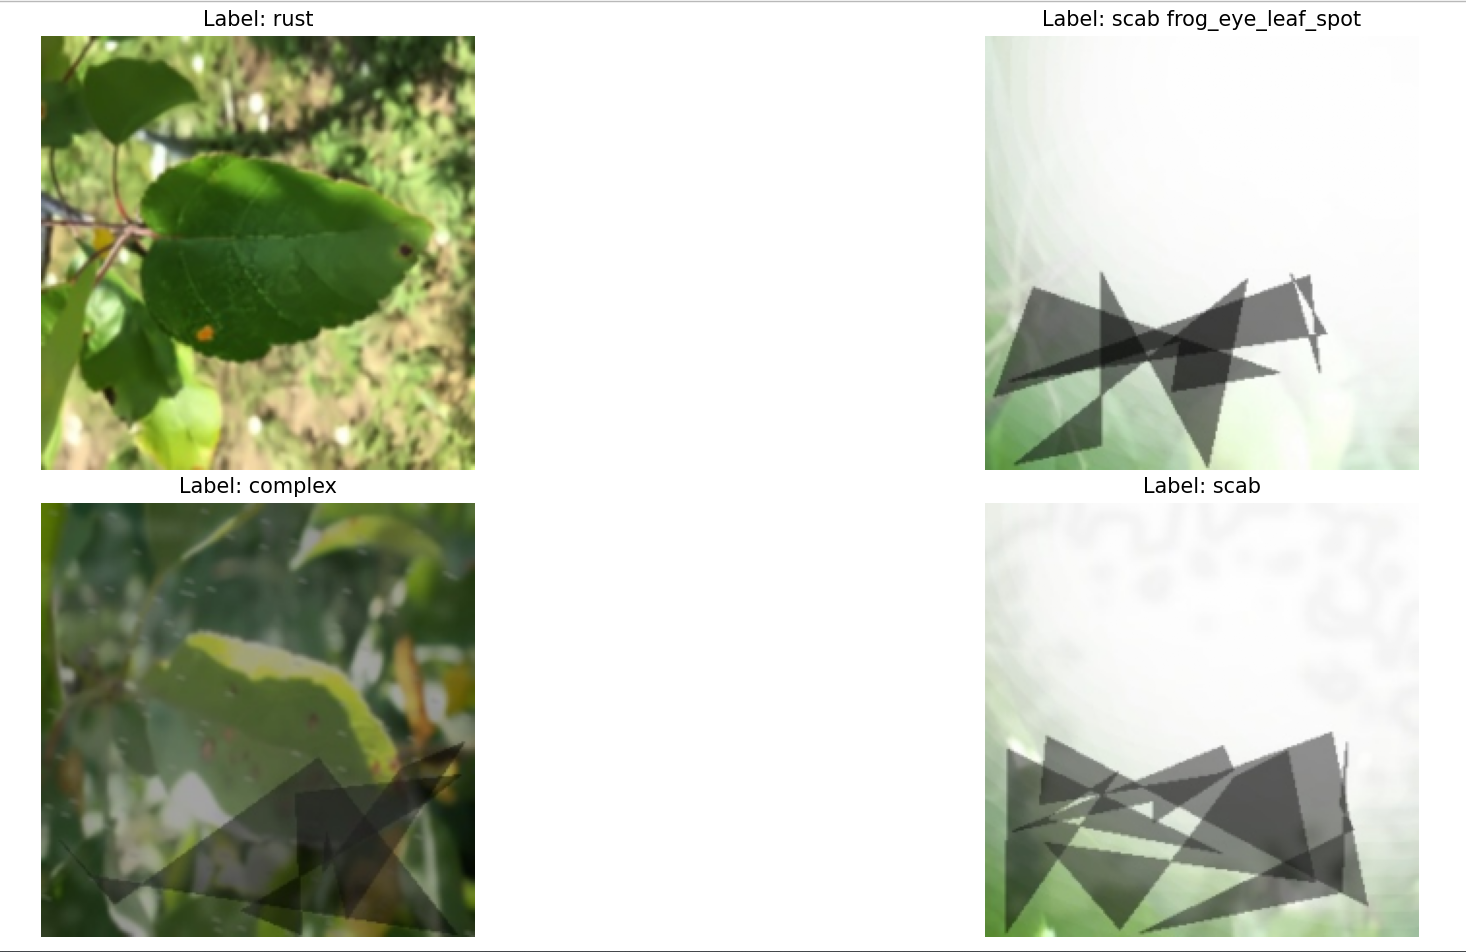
\includegraphics[width=1\columnwidth]{images/image1.png}
    %    in orange color
    \textcolor{orange}{As we can see in the image, the weather-based augmentations have been applied to the original image, simulating different weather conditions.}
    \begin{itemize}
        \item \textbf{Normal Image:} The original image without any modifications.
        \item \textbf{Image with Shadow:} We added a \textcolor{gray}{random shadow} effect for a dynamic look.
        \item \textbf{Image with Fog:} A layer of \textcolor{blue!50}{fog} was introduced to create a misty atmosphere.
        \item \textbf{Image with Rain:} We applied a \textcolor{blue}{rain} effect to simulate a rainy environment.
    \end{itemize}
    
    \end{center}  
    }
    \vspace{0.3in}
\item \textcolor{deepblue}{\textbf{Dataset Split:}} {
    \begin{tcolorbox}[options={colframe=orange},title=Dataset Split]
        \begin{itemize}
            \item \textbf{Training Set:} 80\% of the data.
            \item \textbf{Validation Set:} 10\% of the data.
            \item \textbf{Test Set:} 10\% of the data.
        \end{itemize}
      
    For this, I created a bash file to randomly split the dataset into training, validation, and test sets.\\
    The script ensured that each set had an equal distribution of images across different classes, maintaining the original dataset's class balance.

    \end{tcolorbox}
}
\newpage
\item \textcolor{deepblue}{\textbf{Website Development:}} 
{
    \begin{center}
        \fcolorbox{green}{green!10}
        {
            \parbox{\dimexpr\linewidth-2\fboxsep-2\fboxrule}
            {
                We developed a user-friendly website interface for users to upload images of plant leaves and receive disease classification results. The website included the following features:
                \begin{itemize}
                    \item A home page with an intuitive interface.
                    \item Model page for knowing about the structure and training of the model.
                    \begin{center}
                        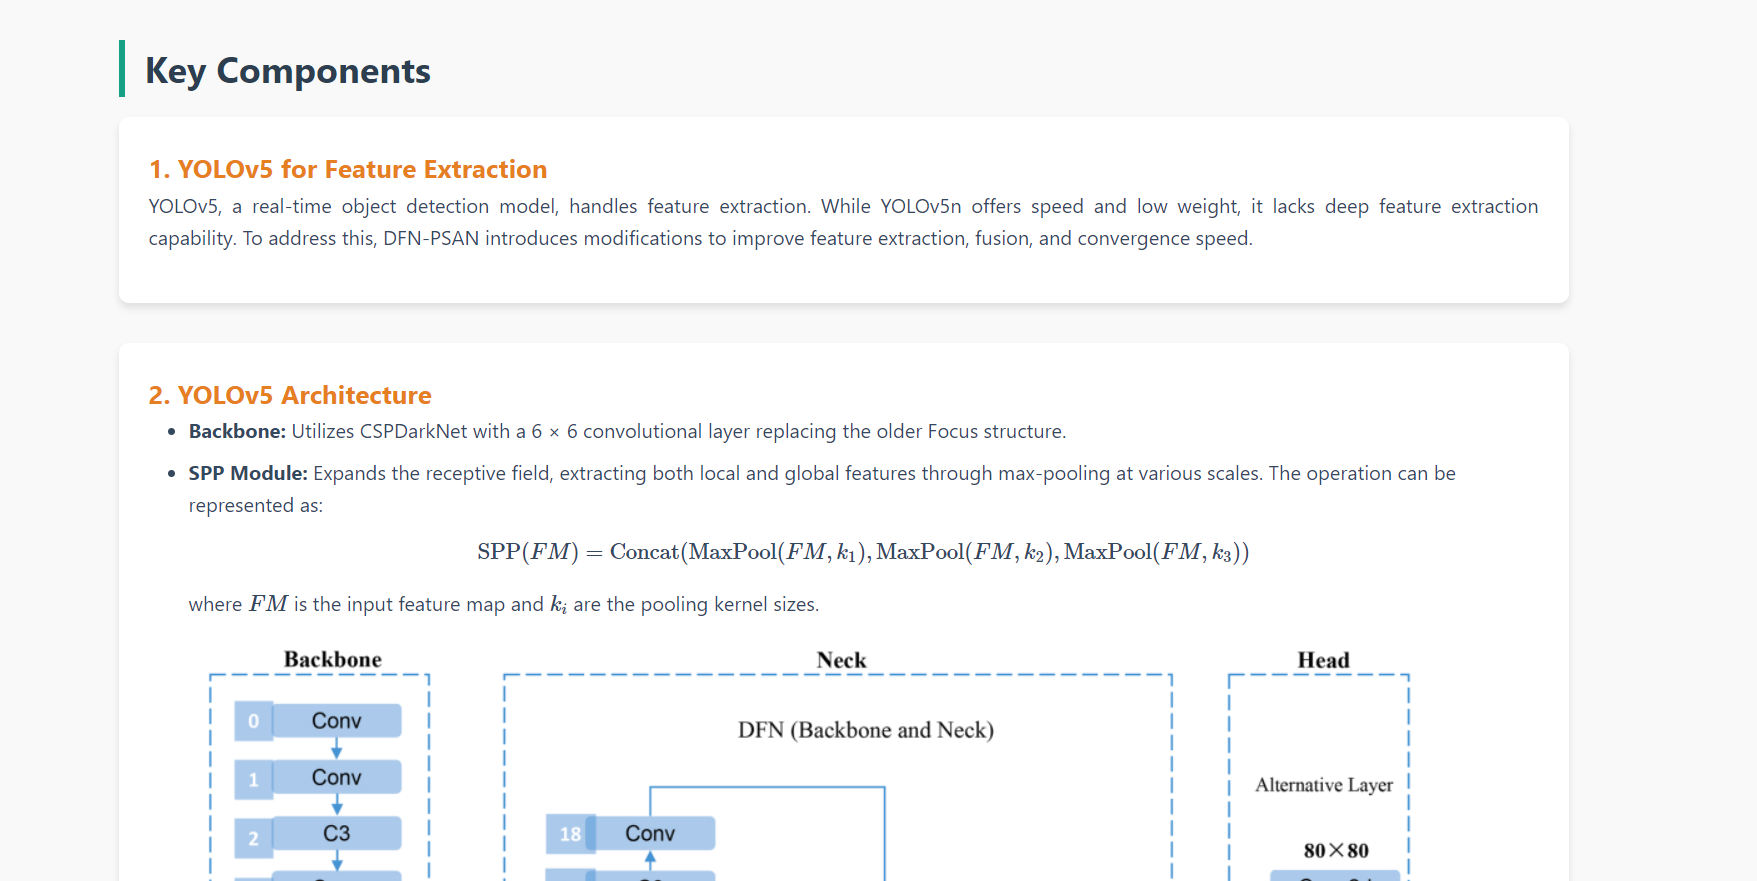
\includegraphics[width=0.8\columnwidth]{images/model.png}
                    \end{center}
                    \item Dataset page for knowing about the dataset used and to download it for personal use.
                    \item An image upload form for users to submit leaf images.
                    \item A results page displaying the predicted disease class.
                \end{itemize}
            }
        }
    \end{center}
   
}

\vspace{0.3in}
\end{enumerate}


\section*{\colorsection{3. Achievements accomplished in this phase.}}
\subsection*{Website Part:}
\subsubsection*{Home interface.}{
    \textcolor{red}{ Home page of our website looks like this.\\
    It has a simple and intuitive interface for users to navigate through different sections of the website.}
   
    \begin{center}
        \fbox{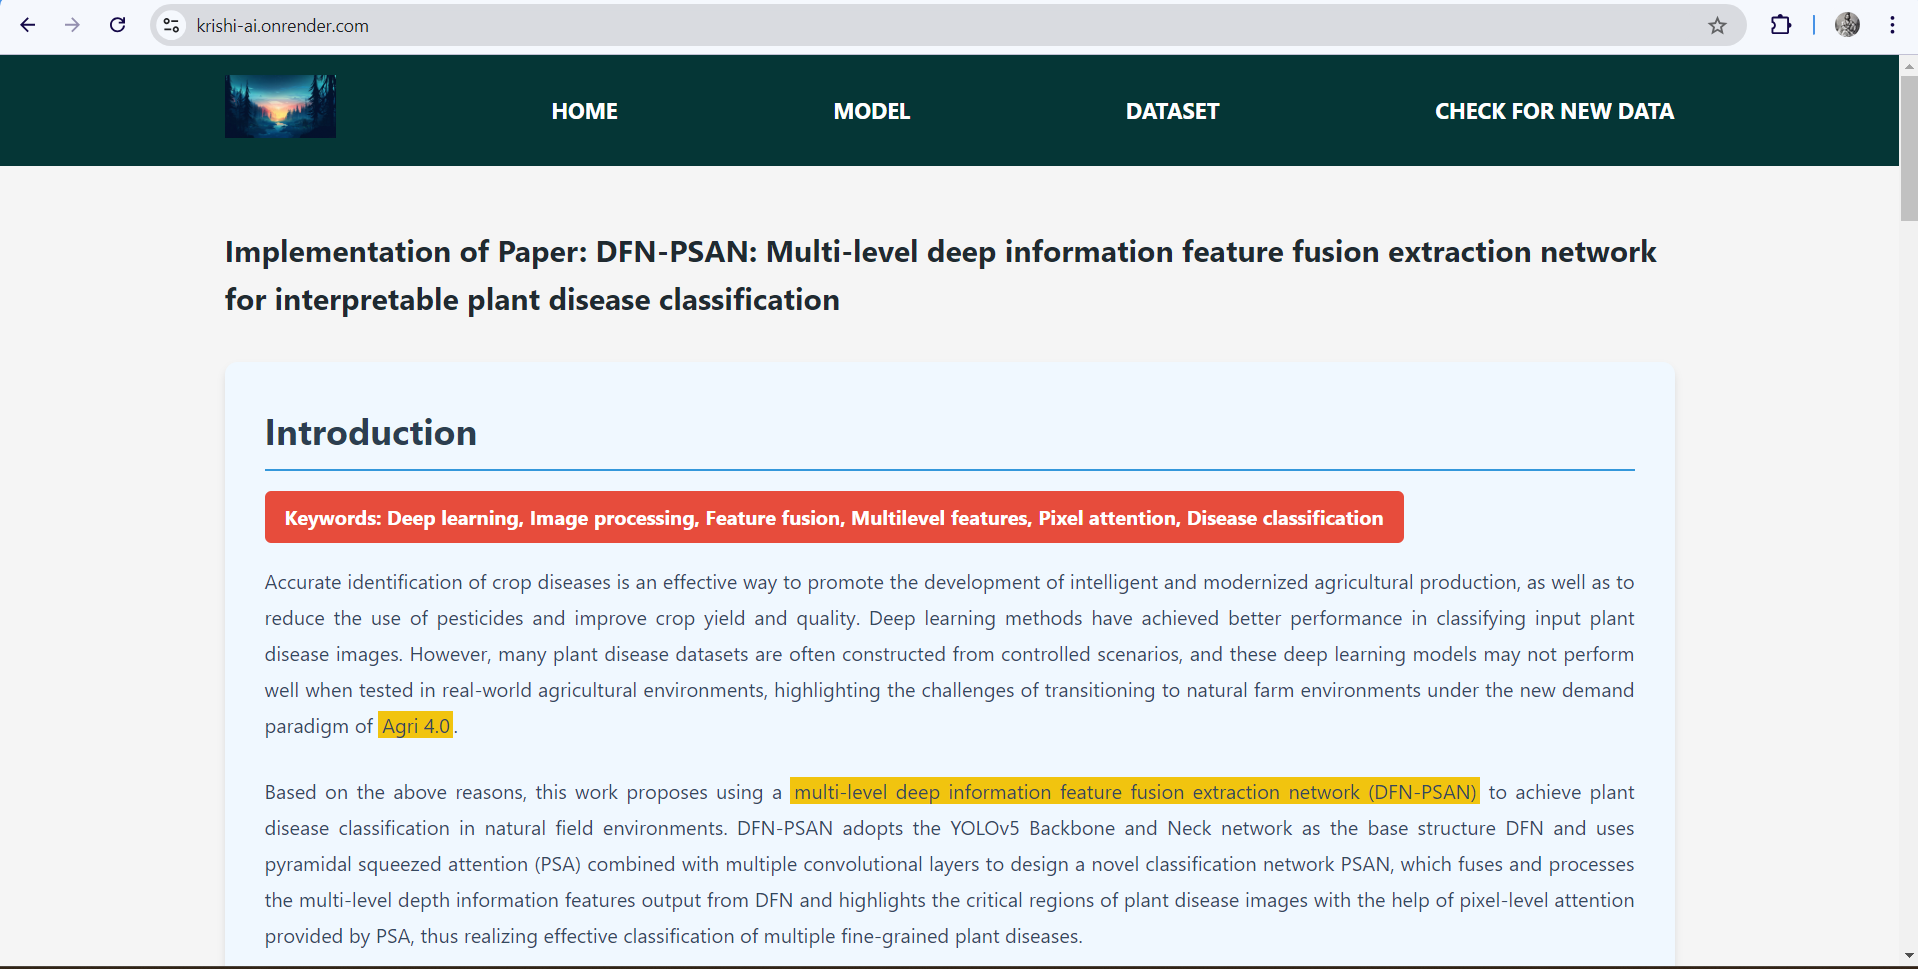
\includegraphics[width=0.9\columnwidth]{images/home_page.png}}
    \end{center}
}
\subsubsection*{Process of Loading Image by the user} 
Any user can upload an image using the following interface:

\begin{center}
    \fcolorbox{black}{white}{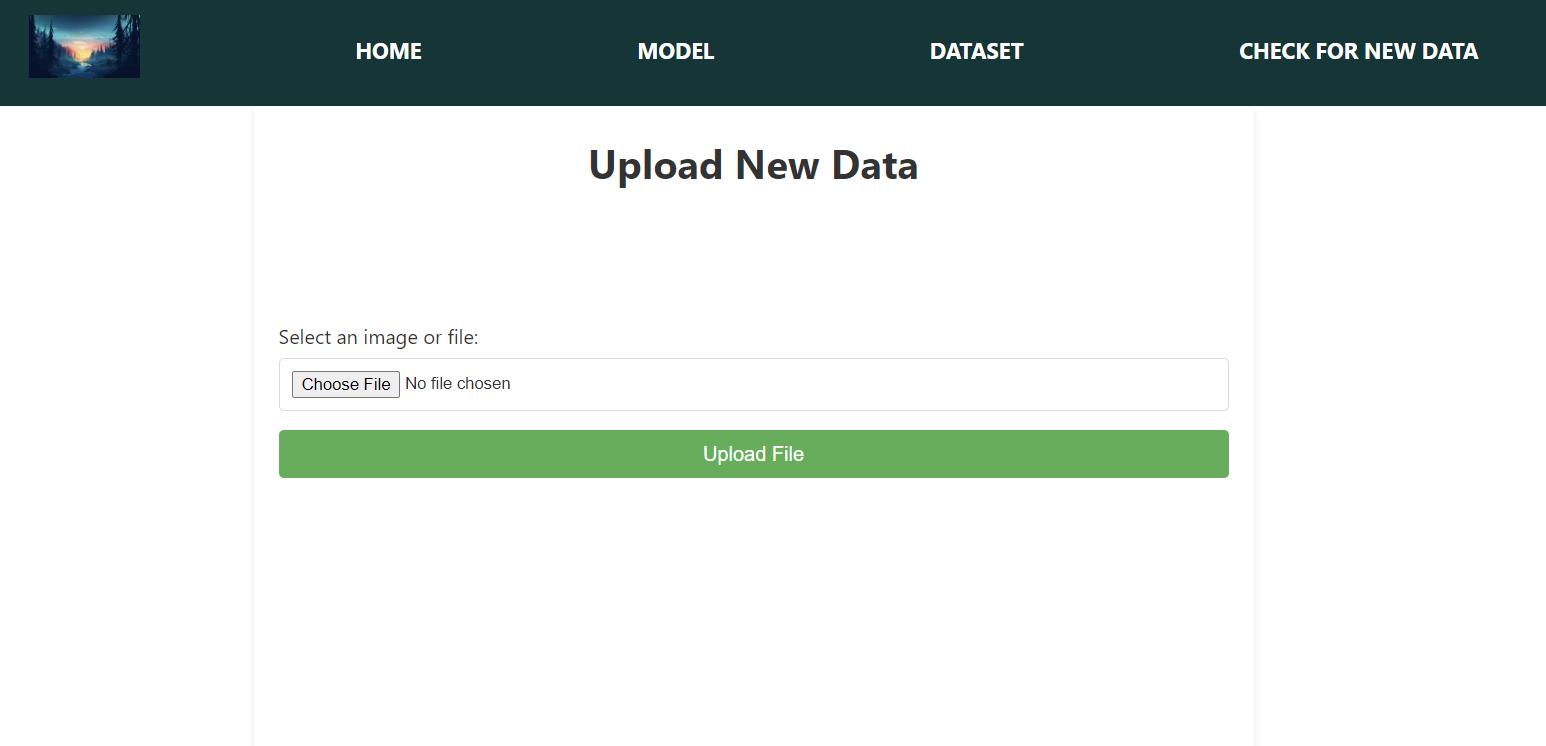
\includegraphics[width=0.9\columnwidth]{images/image4.png}}
    \caption{Form Interface to upload the image of a plant.}
\end{center}

\begin{center}
    \fcolorbox{black}{white}{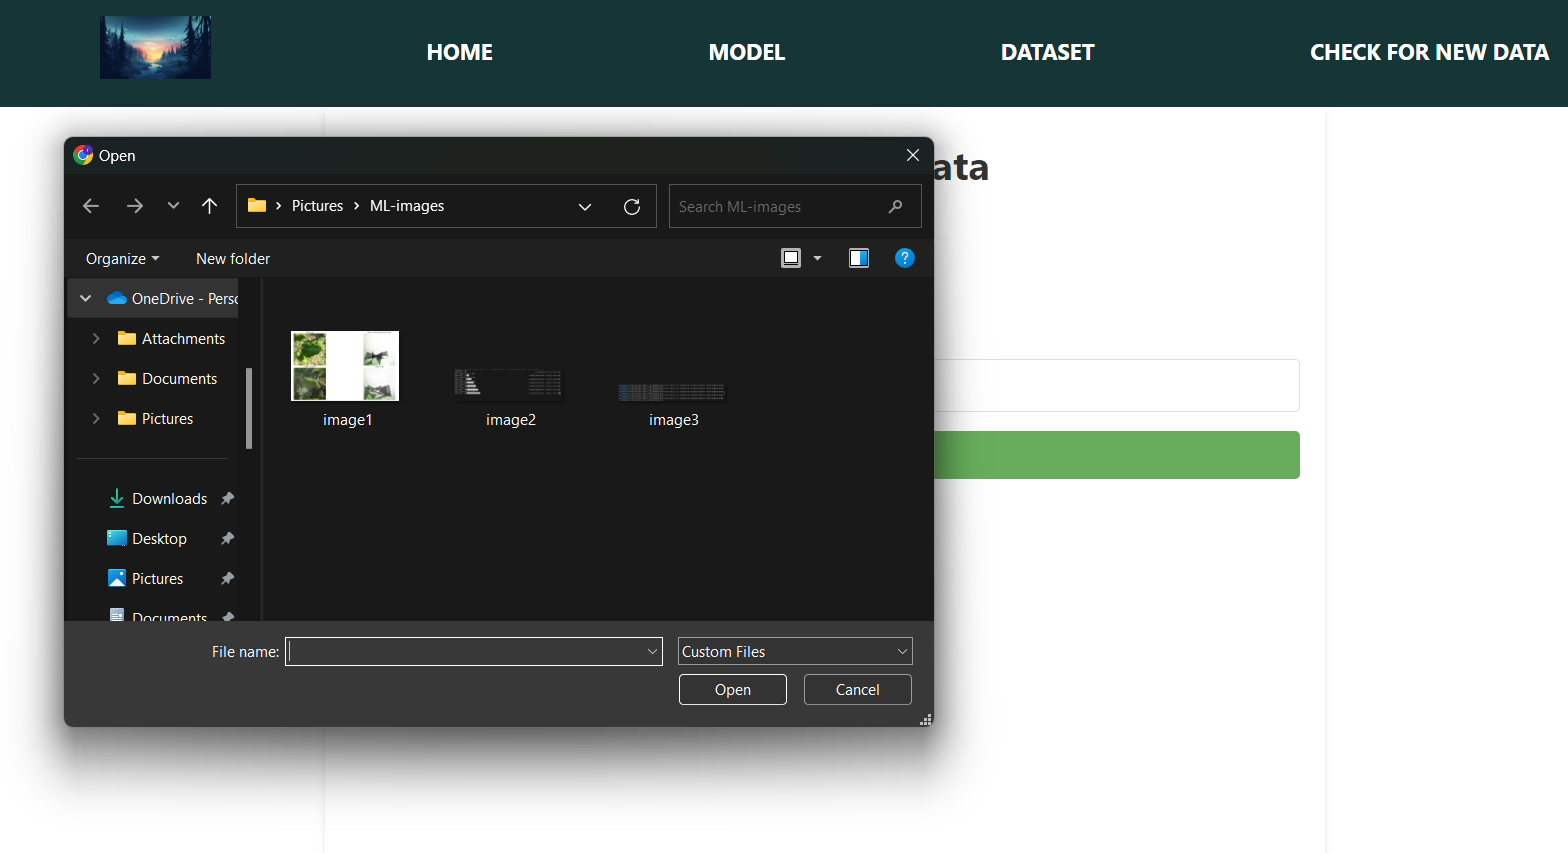
\includegraphics[width=0.9\columnwidth]{images/image5.png}}
    \caption{Image uploaded by the user.}
\end{center}

\subsubsection*{Results Page}
{
    \textcolor{red}{The results page displays the predicted disease class along with the confidence score.}
    \begin{center}
        \fbox{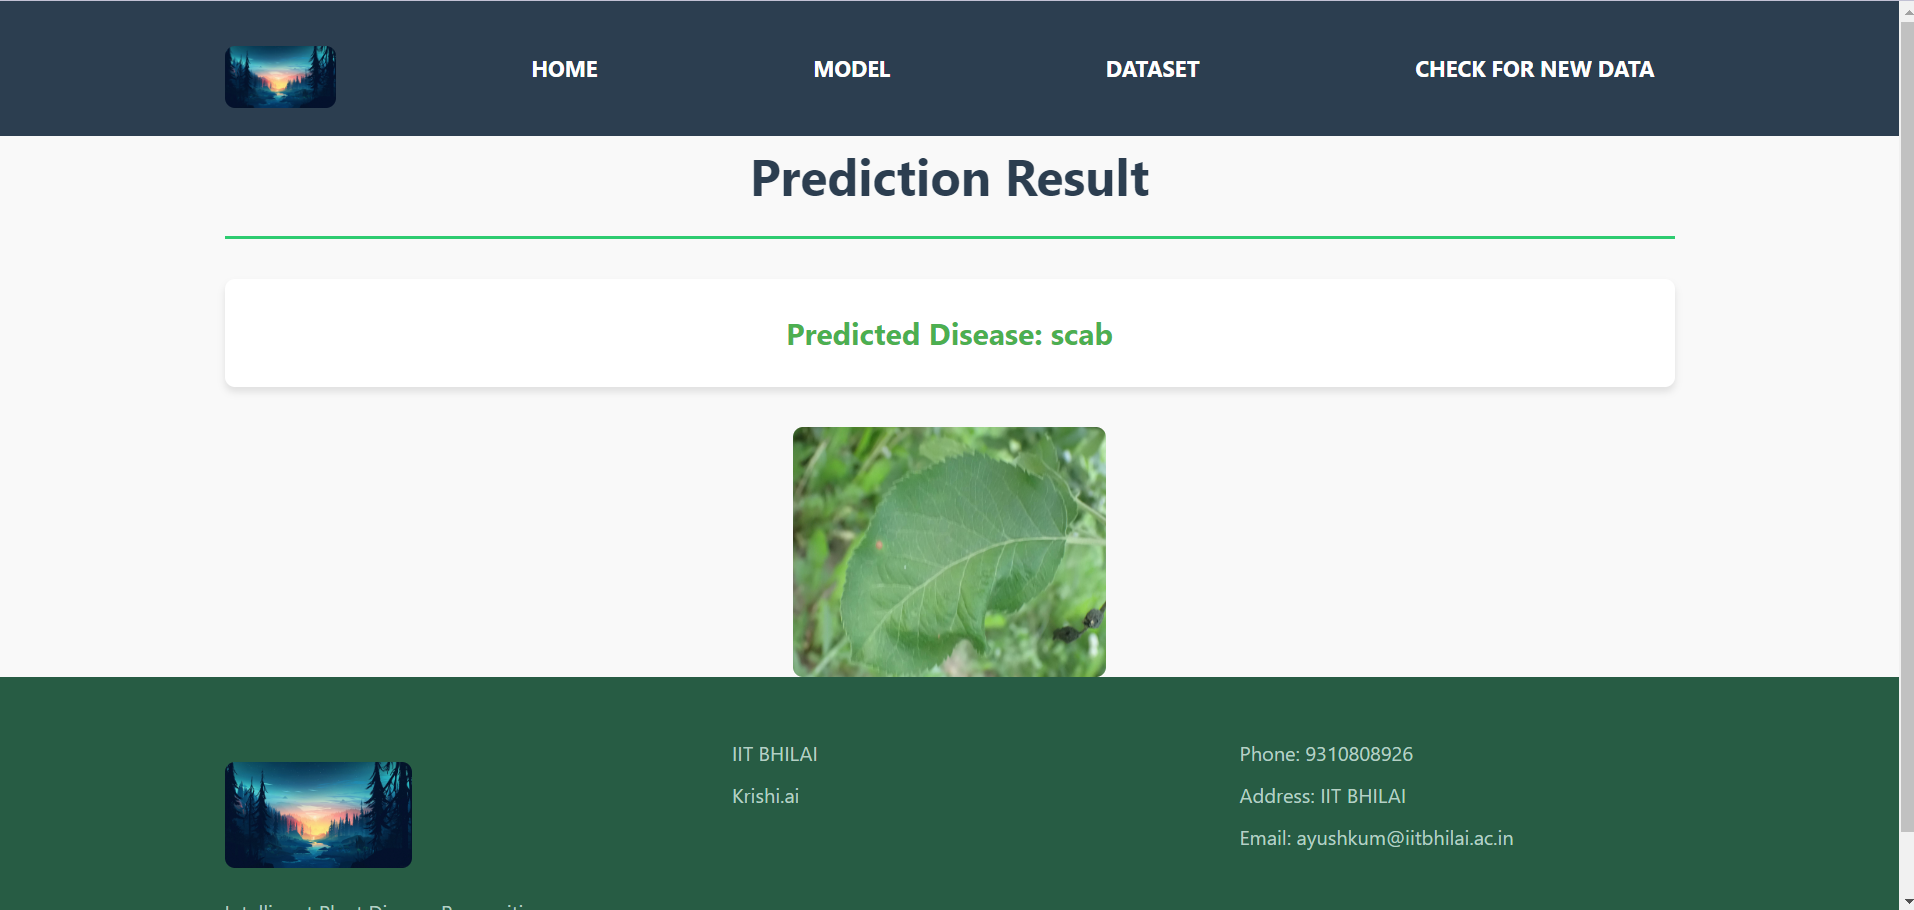
\includegraphics[width=0.9\columnwidth]{images/scab.png}}
    \end{center}
    \large 
    \textcolor{red}{The model predicted the disease as \textbf{Scab}.}
    \begin{center}
        \fbox{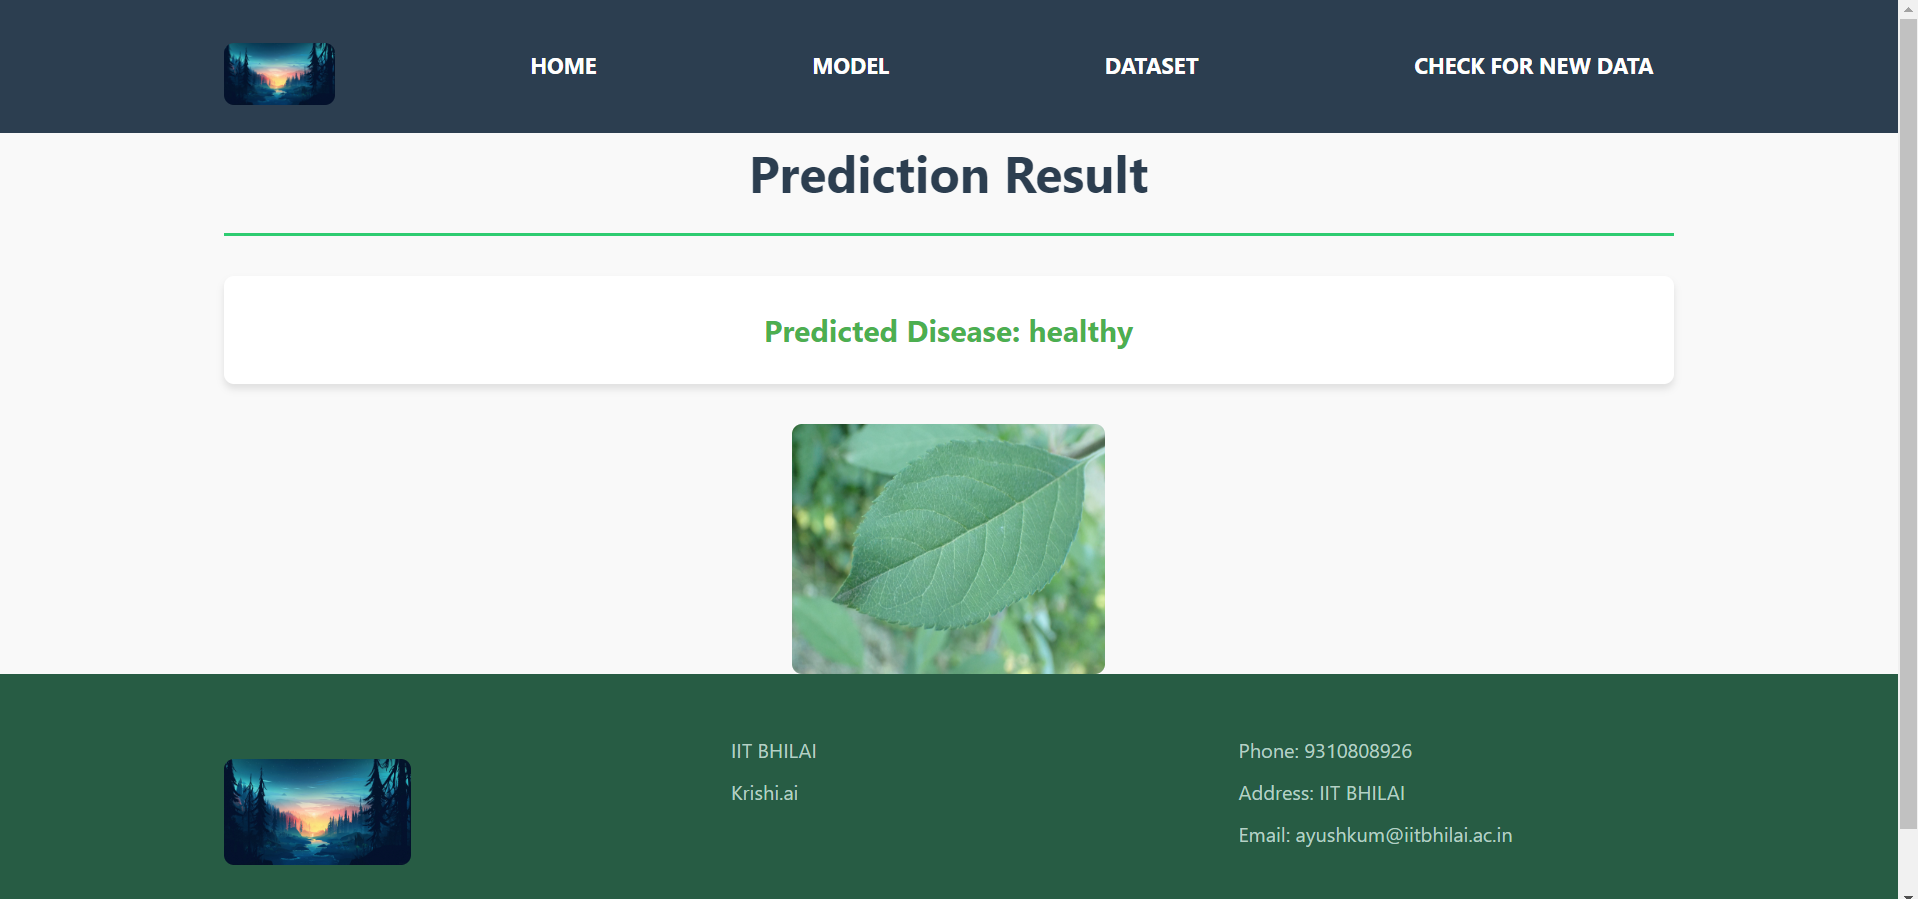
\includegraphics[width=0.9\columnwidth]{images/healthly.png}}
    \end{center}
    \large 
    \textcolor{red}{The confidence score for this prediction is \textbf{healthly}.}
    \normalsize
}


\section*{\colorsection{4. Tasks to be Done}}

\vspace{0.5cm}

\subsection*{\textcolor{deepblue}{Hyperparameter Tuning}}
\textbf{Objective:} \textit{Hyperparameter tuning is a critical step to enhance the model's performance. We will explore different combinations of learning rates, batch sizes, and optimization techniques to find the most effective configuration.}

\vspace{0.2cm}

\textbf{Steps:} 
\begin{itemize}
    \item Explore different hyperparameter combinations using \textbf{grid search} and \textbf{random search}.
    \item Apply cross-validation to ensure consistent model performance across configurations.
\end{itemize}

\vspace{0.5cm}

\subsection*{\textcolor{deepblue}{PSAN Parameter Complexity}}
\textbf{Objective:} \textit{The current configuration of the PSAN (Pyramid Split Attention Network) parameters is overly simplistic. Our goal is to introduce more complexity to better capture high-level features, improving model robustness and accuracy.}

\vspace{0.2cm}

\textbf{Steps:} 
\begin{itemize}
    \item Experiment with deeper layers and refine attention mechanisms.
    \item Adjust split strategies and attention modules to optimize feature extraction.
\end{itemize}

\vspace{0.5cm}

\subsection*{\textcolor{deepblue}{Model Expansion to Other Datasets}}
\textbf{Objective:} \textit{The current model has been trained on only one dataset. We aim to extend the training process to the other two available datasets to ensure generalization across diverse data sources.}

\vspace{0.2cm}

\textbf{Steps:}
\begin{itemize}
    \item Preprocess and augment the additional datasets.
    \item Train the model on new datasets and validate it across all datasets to ensure consistent and accurate results.
\end{itemize}

\vspace{0.5cm}

\subsection*{\textcolor{deepblue}{Generalization for Future Datasets}}
\textbf{Objective:} \textit{To ensure the model can handle new datasets in the future, improving flexibility and adaptability to various data types.}

\vspace{0.2cm}

\textbf{Steps:}
\begin{itemize}
    \item Design a flexible model architecture that can generalize with minimal retraining.
    \item Utilize \textbf{transfer learning} and fine-tuning strategies for incorporating new datasets efficiently.
\end{itemize}

\section*{\colorsection{5. Members Contribution}}

\vspace{0.7cm}

\noindent
\textbf{\textcolor{blue}{Ayush Patel (12240350)}}
\begin{itemize}
    \item \textcolor{blue!80!black}{\textbf{Data Augmentation \& Preprocessing:}} Made data pipeline for performing preprocessing, including image resizing(256 * 256 pixels),\\
    \vspace{0.1in}
    applying \textbf{GaussianBlur}, \textbf{fastNlMeansDenoisingColored},\textbf{convertScaleAbs}\\ and augmentation using \textbf{RandomFog, RandomRain, RandomShadow, RandomSunFlare} to ensure high-quality data for training.
    \vspace{0.1in}
    \item \textcolor{blue!80!black}{\textbf{Data Management:}} Managed dataset versioning (managed all the git related stuffs) and ensured smooth data handling for training and validation.
    \vspace{0.1in}
    \item \textcolor{blue!80!black}{\textbf{Code Optimization:}} Optimized the DFN model's efficiency through mixed-precision training and minimizing redundant computations.
\end{itemize}

\vspace{1cm}

\newpage
\noindent
\textbf{\textcolor{green!60!black}{Ayush Kumar Mishra (12240340)}}
\begin{itemize}
    \item \textcolor{green!80!black}{\textbf{Model Architecture Implementation (DFN):}} Played a key role in implementing the Deep Fusion Network (DFN) backbone, utilizing the YOLOv5 architecture and designing the multi-level feature fusion module.
    \vspace{0.1in}
    \item \textcolor{red!80!black}{\textbf{Model Training \& Evaluation:}} Managed the model training process, including loss function optimization, early stopping, and model evaluation on validation data.
    \vspace{0.1in}
   \item \textcolor{orange!80!black}{\textbf{Splited the data}} Made bash script to split the data into training, validation, and test set randomly acc to config stated in research paper.
   \vspace{0.1in}
    \item \textcolor{green!80!black}{\textbf{Integrating model into flask:}} Integrated the trained model into the Flask server, enabling seamless interaction between the website and the model.
\end{itemize}

\vspace{1cm}

\noindent
\textbf{\textcolor{red!60!black}{Divyanshu Prakash (12240540)}}
\begin{itemize}
    \item \textcolor{red!80!black}{\textbf{Pyramid Squeezed Attention Module (PSA):}} Contributed to integrating and fine-tuning the Pyramid Squeezed Attention Network (PSAN) module for better feature extraction.
    \vspace{0.1in}
    \item \textcolor{red!80!black}{\textbf{Website Development:}} Helped in developing the website interface, designing the homepage, and ensuring the image upload feature for disease classification.
    \vspace{0.1in}
\end{itemize}

\vspace{1cm}

\noindent
\textbf{\textcolor{orange!70!black}{Shivam (12241710)}}
\begin{itemize}
    \item \textcolor{orange!80!black}{\textbf{Project Workflow \& Coordination:}} Led the overall project workflow, assigning tasks, managing deadlines, and ensuring that team members were aligned with their responsibilities.
    \item \textcolor{orange!80!black}{\textbf{Pyramid Squeezed Attention Module (PSA):}} Worked alongside Divyanshu to fine-tune the attention layers in the PSAN module.
    \item \textcolor{red!80!black}{\textbf{Helped in Data Augmentation:}} Helped in implementing weather-based augmentations, including sun flare, rain, shadow, and fog effects.
\end{itemize}

\vspace{1cm}

\noindent
\textbf{\textcolor{purple!60!black}{Ujjwal Raj (12241920)}}
\begin{itemize}
    \item \textcolor{purple!80!black}{\textbf{Website Development:}} Spearheaded the development of the website interface, ensuring proper design and functionality for the disease classification system.
    \item \textcolor{purple!80!black}{\textbf{Deployment:}} Integrated the trained model into the website and managed the deployment pipeline on the Render platform, ensuring user-friendly interaction.
    \item \textcolor{purple!80!black}{\textbf{Model Tuning:}} Focused on hyperparameter tuning to achieve better accuracy by adjusting learning rates, batch sizes, and regularization techniques.
\end{itemize}

\begin{center}
***
\end{center}

\end{document}
